\documentclass{beamer}
\usetheme{metropolis}

\usepackage[ngerman]{babel}
\usepackage[autostyle=true,german=quotes]{csquotes}
\usepackage[linewidth=1pt]{mdframed}
\usepackage{hyperref}
\usepackage{makecell}
\usepackage{pifont}
\usepackage{tikz}
\usetikzlibrary{positioning, calc, arrows, fit, decorations.pathreplacing, shapes, shapes.multipart, snakes}
\usepackage{verbatim}
\usepackage{textcomp}
\usepackage{centernot}
\usepackage{tabularx}
\usepackage{ulem}
%\usepackage{pdfpages}

\batchmode

\hypersetup{
	colorlinks,
	urlcolor=blue,
	linkcolor=black % for ToC
}
\newenvironment{qaa}[1]{
	#1

	\begin{mdframed}
		\small
}{
	\end{mdframed}
}

\newcommand{\true}{\ding{51}}
\newcommand{\false}{\ding{55}}
\newcommand{\code}[1]{
	\begin{mdframed}
		\verbatiminput{#1}
	\end{mdframed}
}


\title{Tutorium 13: Compiler}
% \subtitle{}
\author{Paul Brinkmeier}
\institute{Tutorium Programmierparadigmen am KIT}
\date{8. Februar 2022}

\begin{document}

\begin{frame}
	\titlepage
\end{frame}

\section{Einführung in Compilerbau}

\begin{frame}{Compiler in ProPa}
	\begin{itemize}
		\item Ein bisschen...
		\begin{itemize}
                        \item Lexikalische Analyse
			\item Syntaktische Analyse (Parsen)
			\item \textcolor{gray}{Semantische Analyse, Optimierung}
			\item Codegenerierung
		\end{itemize}
		\pause
		\item Klausur:
		\begin{itemize}
			\item SLL(k)-Form beweisen
			\item Rekursiven Abstiegsparser schreiben/vervollständigen
			\item First/Follow-Mengen berechnen
			\item Java-Bytecode
				% Zeigen: Java-BC-Aufgabe (21SS), Code-Generierung nächste Mittwoch und Freitag (findet noch statt)
		\end{itemize}
	\end{itemize}
\end{frame}

\subsection{Syntaktische Analyse (18WS)}

\begin{frame}{Syntaktische Analyse (18WS)}
	\begin{align*}
		SGML \to & \;\; \textrm{\texttt{< id >}} \;\; Children \;\; \textrm{\texttt{< / >}}\\
		Children \to & \;\; \epsilon \mid SGML \;\; Children
	\end{align*}

	\begin{equation*}
		\{\textrm{\texttt{<id><id></><id></></>}},\;\;\textrm{\texttt{<id></>}},\;\;...\} \in G
	\end{equation*}

	\pause
	\begin{itemize}
		\item Begründen Sie formal, dass die obige Grammatik nicht in $\textrm{SLL}(1)$-Form ist (3P.).
		\pause
		\item Entwickeln Sie für [eine linksfaktorisierte Version der obigen Grammatik] einen rekursiven Abstiegsparser (16P.).
	\end{itemize}
\end{frame}

\begin{frame}{Java-Bytecode (16SS)}
	\footnotesize
	Übersetzen Sie folgenden Java-Programmausschnitt in Java-Bytecode (10P.):

	\code{code/bytecode16ss.java}

	\pause
	Hinweise:

	\begin{itemize}
		\item Codeerzeugung für bedingte Sprünge: Folien 447ff.
		\item Um eine Bedingung der Form \texttt{!cond} zu übersetzen, reicht es, \texttt{cond} zu übersetzen und die Sprungziele anzupassen.
	\end{itemize}
\end{frame}

\section{Compiler}

\subsection{Motivation}

\begin{frame}{Compiler: Motivation}
	\begin{itemize}
		\item Maschine(-nmodell) versteht i.d.R. eingeschränkten Instruktionssatz
		\item $\leadsto$ Programme in Maschinensprache sind schwer les-/schreibbar
		\pause
		\item Also: Erfinde einfacher zu Schreibende ($\approx$ mächtigere) Sprache, die dann in die Sprache der Maschine übersetzt wird.
		\item Diesen Übersetzungsschritt sollte optimalerweise ein Programm erledigen, da wir sonst auch einfach direkt Maschinensprache-Programme schreiben können.
	\end{itemize}
\end{frame}

\begin{frame}{Compiler}
	\begin{itemize}
		\item Übersetzer für formale Sprachen nennt man \emph{Compiler}
		\item Beispiele:
		\begin{itemize}
			\item C, Haskell, Rust, Go $\to$ X86
			\item Java, Scala, Kotlin $\to$ Java-Bytecode
			\item TypeScript $\to$ JavaScript/WebAssembly
		\end{itemize}
		\pause
		\item Single-pass vs. Multi-pass
		\begin{itemize}
			\item Single-pass: Eingabe wird einmal gelesen, Ausgabe währenddessen erzeugt (ältere Compiler)
			\item Multi-pass: Eingabe wird in Zwischenschritten in verschiedene Repräsentationen umgewandelt
			\begin{itemize}
				\item Quellsprache, Tokens, AST, Zwischensprache, Zielsprache
			\end{itemize}
		\end{itemize}
	\end{itemize}
\end{frame}

\subsection{Lexikalische Analyse}

\begin{frame}{Lexikalische Analyse}
	\begin{columns}
		\begin{column}{0.5\textwidth}
			\code{code/lexinput.java}
		\end{column}
		\begin{column}{0.5\textwidth}
			\code{code/lexoutput.java}
		\end{column}
	\end{columns}

	\begin{itemize}
		\item Lexikalische Analyse (Tokenisierung) verarbeitet eine Zeichensequenz in eine Liste von \emph{Tokens}.
		\item Tokens sind Zeichengruppen, denen eine Semantik innewohnt:
		\begin{itemize}
			\item \texttt{int} --- Typ einer Ganzzahl
			\item \texttt{=} --- Zuweisungsoperator
			\item \texttt{x1} --- Variablen- oder Methodenname
			\item \texttt{123} --- Literal einer Ganzzahl
			\item \texttt{"123"} --- String-Literal
			\item etc.
		\end{itemize}
		\item Lösbar mit regulären Ausdrücken, Automaten
	\end{itemize}
\end{frame}

\subsection{Syntaktische Analyse}

\begin{frame}{Syntaktische Analyse}
	\begin{itemize}
                \item Syntaktische Analyse stellt die unterliegende (Baum-)Struktur der bisher linear gelesenen Eingabe fest:
		\begin{itemize}
			\item Blockstruktur von Programmen
			\item Baumstruktur von HTML-Dateien
			\item Header + Inhalt-Struktur von Mails
			\item Verschachtelte arithmetische Ausdrücke
		\end{itemize}
		\item Syntaktische Analyse ist das größte Compiler-Thema in PP.
		\pause
		\item Übliche Vorgehensweise (in PP):
		\begin{itemize}
			\item Grammatik $G$ erfinden
			\item Ggf. $G$ in andere Form $G'$ bringen
			\item Rekursiven Abstiegsparser für $G'$ implementieren
		\end{itemize}
		\item Alternativ: Parser-Kombinatoren, Yacc, etc.
	\end{itemize}
\end{frame}

\begin{frame}{Beispiel: Arithmetische Ausdrücke}
  \begin{center}
    \textcolor<1>{red}{\texttt{a+a+b}} \hfill \textcolor<2>{red}{\texttt{a*c+b}} \hfill \textcolor<3>{red}{\texttt{a*c+b*d}}
  \end{center}

    \begin{itemize}
      \item Zu beachten: Punkt-vor-Strich (Präzedenz), Klammerung, etc.
      \item Nicht mehr mit regulären Ausdrücken lösbar
      \item Beispielgrammatik:
    \end{itemize}

    \begin{columns}
      \begin{column}{0.5\textwidth}
        \begin{align*}
          E \to & \; E \;\; \texttt{+} \;\; E \\
           \mid & \; E \;\; \texttt{*} \;\; E \\
           \mid & \; \texttt{(} \;\; E \;\; \texttt{)} \\
           \mid & \; \texttt{id}
        \end{align*}
      \end{column}
      \begin{column}{0.5\textwidth}
        \only<1>{
          \begin{tikzpicture}[level distance=10mm, sibling distance=10mm]
            \node {E}
              child {
                node {E}
                  child {
                    node {E}
                      child {node {\texttt{id[a]}}}
                  }
                  child {node {\texttt{+}}}
                  child {
                    node {E}
                      child {node {\texttt{id[a]}}}
                  }
              }
              child {
                node {\texttt{+}}
              }
              child {
                node {E}
                  child {
                    node {\texttt{id[b]}}
                  }
              }
            ;
          \end{tikzpicture}
        }
        \only<2>{
          \begin{tikzpicture}[level distance=10mm, sibling distance=10mm]
            \node {E}
              child {
                node {E}
                  child {
                    node {E}
                      child {node {\texttt{id[a]}}}
                  }
                  child {node {\texttt{*}}}
                  child {
                    node {E}
                      child {node {\texttt{id[c]}}}
                  }
              }
              child {
                node {\texttt{+}}
              }
              child {
                node {E}
                  child {
                    node {\texttt{id[b]}}
                  }
              }
            ;
          \end{tikzpicture}
        }
        \only<3>{
          \begin{tikzpicture}[level distance=7.5mm, sibling distance=10mm]
            \node {E}
              child {
                node {E}
                  child {
                    node {E}
                      child {node {\texttt{id[a]}}}
                  }
                  child {node {\texttt{*}}}
                  child {
                    node {E}
                      child {node {E}
                        child {node {\texttt{id[c]}}}
                      }
                      child {node {\texttt{+}}}
                      child {node {E}
                        child {node {\texttt{id[b]}}}
                      }
                  }
              }
              child {
                node {\texttt{*}}
              }
              child {
                node {E}
                  child {
                    node {\texttt{id[d]}}
                  }
              }
            ;
          \end{tikzpicture}
        }
      \end{column}
    \end{columns}
\end{frame}

\begin{frame}{Beispiel: Mathematische Ausdrücke}
	\begin{equation*}
          E \to \; E \;\; \texttt{+} \;\; E \;
           \mid \; E \;\; \texttt{*} \;\; E \;
           \mid \; \texttt{(} \;\; E \;\; \texttt{)} \;
           \mid \; \texttt{id}
	\end{equation*}

        \begin{center}
          \texttt{a*c+b}
        \end{center}

	\pause

        \begin{columns}
          \begin{column}{0.5\textwidth}
            \begin{tikzpicture}[level distance=7.5mm, sibling distance=10mm]
              \node {E}
                child {
                  node {E}
                    child {
                      node {E}
                        child {node {\texttt{id[a]}}}
                    }
                    child {node {\texttt{*}}}
                    child {
                      node {E}
                        child {node {\texttt{id[c]}}}
                    }
                }
                child {
                  node {\texttt{+}}
                }
                child {
                  node {E}
                    child {
                      node {\texttt{id[b]}}
                    }
                }
              ;
            \end{tikzpicture}
          \end{column}
          \begin{column}{0.5\textwidth}
            \begin{tikzpicture}[level distance=7.5mm, sibling distance=10mm]
              \node {E}
                child {
                  node {E}
                    child {
                      node {\texttt{id[a]}}
                    }
                }
                child {
                  node {\texttt{*}}
                }
                child {
                  node {E}
                    child {
                      node {E}
                        child {node {\texttt{id[c]}}}
                    }
                    child {node {\texttt{+}}}
                    child {
                      node {E}
                        child {node {\texttt{id[b]}}}
                    }
                }
              ;
            \end{tikzpicture}
          \end{column}
        \end{columns}

	\begin{itemize}
          \item Grammatik nicht eindeutig $\leadsto$ schlecht
          \item Grammatik garantiert nicht Punkt-vor-Strich $\leadsto$ schlecht
          \item Grammatik ist linksrekursiv $\leadsto$ nicht einfach zu parsen $\leadsto$ schlecht
	\end{itemize}
\end{frame}

\begin{frame}{Grammar Engineering 1 --- Präzedenz}
  \begin{equation*}
    E \to \; E \;\; \texttt{+} \;\; E \;
     \mid \; E \;\; \texttt{*} \;\; E \;
     \mid \; \texttt{(} \;\; E \;\; \texttt{)} \;
     \mid \; \texttt{id}
  \end{equation*}

  \begin{itemize}
    \item Punkt-vor-Strich (\enquote{Operatorpräzedenz}) wird von dieser naiven Grammatik nicht beachtet.
    \item Lösung: Ein Nichtterminal pro Präzedenzstufe:
    \begin{itemize}
      \item \emph{Summen} von \emph{Produkten} von \emph{Atomen}.
      \item Herkömmliche Begriffe: Ausdruck, Term und Faktor.
    \end{itemize}
  \end{itemize}

  \begin{alignat*}{2}
    & Expr   & \; \to \; & Expr \; \texttt{+} \; Term \\
          && \mid \;\; & Term \\
    & Term   & \; \to \; & Term \; \texttt{+} \; Factor \\
            && \mid \;\; & Factor \\
    & Factor & \; \to \; & \texttt{(} \; Expr \; \texttt{)} \; \mid \; \texttt{id}
  \end{alignat*}
\end{frame}

\begin{frame}{Welche Art von Grammatik wollen wir denn genau?}
  \begin{columns}
    \begin{column}{0.5\textwidth}
      \begin{tikzpicture}[
        box/.style={
          draw=black,
          rounded corners
        },
        every fit/.style={
          inner sep=2mm
        },
        node distance=3mm
      ]
        \node[box] (rg) {RG};
        \node[below=of rg] (sll) {SLL(1)};
        \node[box,fit=(rg) (sll),draw=blue] (b1) {};

        \node[right=of b1] (lr) {LR(1)};
        \node[box,fit=(b1) (lr)] (b3) {};

        \node[below=of b3] (dcfg) {DCFG};
        \node[box,fit=(b3) (dcfg)] (b4) {};

        \node[below=of b4] (cfg) {CFG};
        \node[box,fit=(b4) (cfg)] {};
      \end{tikzpicture}
    \end{column}
    \begin{column}{0.5\textwidth}
      \footnotesize

      \begin{itemize}
        \item CFG-Parsen ist i.A. in $O(n^3)$, bspw. Earley-Algorithmus.
        \item Reguläre Grammatiken ($\approx$ reg. Sprachen) sind uns nicht mächtig genug.
        \item \textcolor{red}{L}\textcolor{blue}{R}: \textcolor{red}{Left-to-right}, \textcolor{blue}{Rightmost}
        \item \textcolor{red}{L}\textcolor{blue}{L}: \textcolor{red}{Left-to-right}, \textcolor{blue}{Leftmost}
        \item SLL-Parsing $\in O(n)$
      \end{itemize}
    \end{column}
  \end{columns}

  \vspace{1cm}
  \center
  CFG: Context-Free Grammar/Kontextfreie Grammatik
\end{frame}

\begin{frame}{Grammar Engineering 2 --- Linksrekursion eliminieren}
  \begin{columns}
    \begin{column}{0.5\textwidth}
      \begin{alignat*}{2}
        & Expr   & \; \to \; & Expr \; \texttt{+} \; Term \\
              && \mid \;\; & Term \\
        & Term   & \; \to \; & Term \; \texttt{+} \; Factor \\
                && \mid \;\; & Factor \\
        & Factor & \; \to \; & \texttt{(} \; Expr \; \texttt{)} \; \mid \; \texttt{id}
      \end{alignat*}

    \end{column}
    \begin{column}{0.5\textwidth}
      \begin{figure}
        \begin{tikzpicture}[
          level distance=7.5mm,
          sibling distance=15mm
        ]
          \node {Expr}
            child {
              node {Expr}
                child {
                  node {Expr}
                    child {
                      node {...}
                    }
                    child {node {Term}}
                }
                child {node {Term}}
            }
            child {node {Term}}
          ;
        \end{tikzpicture}
      \end{figure}
    \end{column}
  \end{columns}

  \vfill

  Problem: Die Linksableitung des Symbols $Expr$ in dieser Grammatik ist eine endlose Schleife.
\end{frame}

\begin{frame}{Grammar Engineering 2 --- Linksrekursion eliminieren}
  \begin{columns}
    \begin{column}{0.5\textwidth}
      \begin{alignat*}{2}
        & Expr   & \; \to \; & Expr \; \texttt{+} \; Term \\
              && \mid \;\; & Term \\
        & Term   & \; \to \; & Term \; \texttt{+} \; Factor \\
                && \mid \;\; & Factor \\
        & Factor & \; \to \; & \texttt{(} \; Expr \; \texttt{)} \; \mid \; \texttt{id}
      \end{alignat*}

    \end{column}
    \begin{column}{0.5\textwidth}
      \begin{alignat*}{2}
        & Expr   & \; \to \; & \; Term \; Expr' \\
        & Expr'  & \; \to \; & \; \texttt{+} \; Term \; Expr' \\
                && \mid \;\; & \; \epsilon \\
        & Term   & \; \to \; & \; Term \; Expr' \\
        & Term'  & \; \to \; & \; \texttt{*} \; Factor \; Term' \\
                && \mid \;\; & \; \epsilon \\
        & Factor & \; \to \; & \texttt{(} \; Expr \; \texttt{)} \; \mid \; \texttt{id}
      \end{alignat*}
    \end{column}
  \end{columns}

  \vfill

  \only<1>{
    Lösung: Linksrekursion eliminieren, durch folgendes Umschreiben der Grammatik:
  }

  \only<2>{
  \begin{columns}
    \begin{column}{0.5\textwidth}
      \begin{alignat*}{2}
        & Sym   & \; \to \; & Sym \; \alpha \\
               && \mid \;\; & \beta
      \end{alignat*}

    \end{column}
    \begin{column}{0.5\textwidth}
      \begin{alignat*}{2}
        & Sym   & \; \to \; & \beta \; Sym' \\
        & Sym'  & \; \to \; & \alpha \; Sym' \\
               && \mid \;\; & \epsilon
      \end{alignat*}
    \end{column}
  \end{columns}
  }
\end{frame}

\begin{frame}{Verbesserte Grammatik}
  \begin{alignat*}{2}
    & E      & \; \to \; & \; T \; EList \\
    & EList  & \; \to \; & \; \texttt{+} \; T \; EList \\
            && \mid \;\; & \; \epsilon \\
    & T      & \; \to \; & \; T \; EList \\
    & TList  & \; \to \; & \; \texttt{*} \; F \; TList \\
            && \mid \;\; & \; \epsilon \\
    & F      & \; \to \; & \texttt{(} \; E \; \texttt{)} \; \mid \; \texttt{id}
  \end{alignat*}

  \begin{itemize}
    \item Grammatik ist eindeutig \true
    \item Grammatik erzeugt nur korrekte Terme \true
    \item Grammatik enthält keine Linksrekursion \true
  \end{itemize}
\end{frame}

\begin{frame}{First-/Followmenge, Indizmenge}
	\footnotesize

	\begin{align*}
		EList \to & \;\; \epsilon \mid \textrm{\texttt{+}} \;\; T \;\; EList \mid \textrm{\texttt{-}} \;\; T \;\; EList
	\end{align*}
	
	Wie können wir bspw. bei $EList$ entscheiden, welche Produktion anzuwenden ist?
	\pause
	\begin{itemize}
		\item $\leadsto$ definiere \emph{Indizmenge} $IM_k(A \to \alpha) = \textrm{First}_k(\alpha \textrm{Follow}_k(A))$
		\item Wenn nächste $k$ Token in $IM_k(EList \to \phi)$ $\leadsto$ weiter mit $\phi$
		\pause
		\item $IM_1(EList \to \; \epsilon) = \textrm{First}_1(\epsilon \textrm{Follow}_1(EList)) = \{ \textrm{\texttt{)}}, \textrm{\texttt{\#}} \}$
		\item $IM_1(EList \to \; \textrm{\texttt{+}} \;\; T \;\; EList) = \textrm{First}_1(\textrm{\texttt{+}} \; T \; EList \; \textrm{Follow}_1(EList)) = \{ \textrm{\texttt{+}} \}$
		\item $IM_1(EList \to \; \textrm{\texttt{-}} \;\; T \;\; EList) = \textrm{First}_1(\textrm{\texttt{-}} \; T \; EList \; \textrm{Follow}_1(EList)) = \{ \textrm{\texttt{-}} \}$
		\pause
		\item $\textrm{First}_k(A)$: Menge an möglichen ersten $k$ Token in $A$
		\item $\textrm{Follow}_k(A)$: Menge an möglichen ersten $k$ Token nach $A$
	\end{itemize}
\end{frame}

\begin{frame}{SLL-Kriterium}
	Grammatik ist in $\textrm{SLL}(k)$-Form\\
	$:\Leftrightarrow \forall A \to \alpha, A \to \beta \in P: IM_k(A \to \alpha) \cap IM_k(A \to \beta) = \emptyset$

	\begin{itemize}
		\item $\textrm{SLL}(k)$: Bei jedem Nichtterminal muss die zu wählende Produktion an den nächsten $k$ Token wählbar sein.
		\item Nichtterminale mit nur einer Produktion sind hier irrelevant
		\item Schwierig daran: $\textrm{Follow}$-Mengen berechnen
	\end{itemize}
	\pause
	\begin{align*}
		E \to & \;\; E \;\; \textrm{\texttt{+}} \;\; T \mid E \;\; \textrm{\texttt{-}} \;\; T \mid T\\
		T \to & \;\; T \;\; \textrm{\texttt{*}} \;\; F \mid T \;\; \textrm{\texttt{/}} \;\; F \mid F\\
		F \to & \;\; \textrm{\texttt{num}} \; | \; \textrm{\texttt{(}} \;\; E \;\; \textrm{\texttt{)}}
	\end{align*}
	
	\begin{itemize}
		\item Begründet formal, dass obige Grammatik nicht $\textrm{SLL}(1)$.
		\item Berechnet $\textrm{Follow}_1(N)$ für $N \in \{ E, T, F \}$.
	\end{itemize}
\end{frame}

\begin{frame}{Rekursive Abstiegsparser}
	\footnotesize
	\begin{align*}
		E     \to & \;\; T \;\; EList\\
		EList \to & \;\; \epsilon \mid \textrm{\texttt{+}} \;\; T \;\; EList \mid \textrm{\texttt{-}} \;\; T \;\; EList\\
		T     \to & \;\; F \;\; TList\\
		TList \to & \;\; \epsilon \mid \textrm{\texttt{*}} \;\; F \;\; TList \mid \textrm{\texttt{/}} \;\; F \;\; TList\\
		F \to & \;\; \textrm{\texttt{num}} \; | \; \textrm{\texttt{(}} \;\; E \;\; \textrm{\texttt{)}}
	\end{align*}
	\begin{itemize}
		\item Yay, unsere Grammatik hat jetzt $\textrm{SLL}(1)$-Form!
		\item Aber was bringt das?
		\pause
		\item $G$ ist jetzt einfach ausprogrammierbar:
		\begin{itemize}
			\item 1 Methode per Nichtterminal: \texttt{parseE()}, \texttt{parseEList()}, ...
			\item \texttt{Token[k]}-Instanzattribut für $k$ langen Lookahead
			\item \texttt{expect(TokenType)}-Methode, um Token zu verarbeiten
		\end{itemize}
	\end{itemize}
\end{frame}

\subsection{Semantische Analyse/Optimierung}

\begin{frame}{Semantische Analyse}
	\begin{itemize}
		\item PP beschäftigt sich (bis auf Typinferenz) nur kurz mit semantischer Analyse
		\item Typchecks/-inferenz, Namensanalyse
		\item $\leadsto$ weiterführende (Master-)Vorlesungen am IPD
	\end{itemize}
\end{frame}

\begin{frame}{Optimierung}
  \begin{itemize}
    \item Moderne Compiler haben i.d.R. (mindestens) eine Zwischensprache, bspw.
    \begin{itemize}
      \item GCC: Generic, GIMPLE, RTL
      \item LLVM, libFirm
      \item GHC: Core, STG
    \end{itemize}
    \item Vorteil: Optimierungen müssen nur einmal implementiert werden
  \end{itemize}
\end{frame}

\subsection{Zwei Beispiele}

\begin{frame}{Beispiel: GCC}
  \begin{figure}
    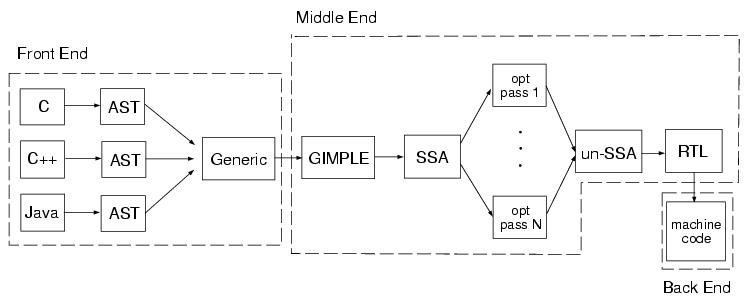
\includegraphics[width=\textwidth]{images/gcc.jpg}
  \end{figure}

  \begin{itemize}
    \item Generic: Sprachunabhängiger Output des Frontend
    \item GIMPLE: Für Optimierungen (SSA: Spezielle Form)
    \item RTL: Für Registerallokation, Instruktionsauswahl
    \item Ca. 15 Mio. Zeilen Code (2019, laut Wikipedia)
  \end{itemize}
\end{frame}

\begin{frame}{Beispiel: GHC}
  \begin{figure}
    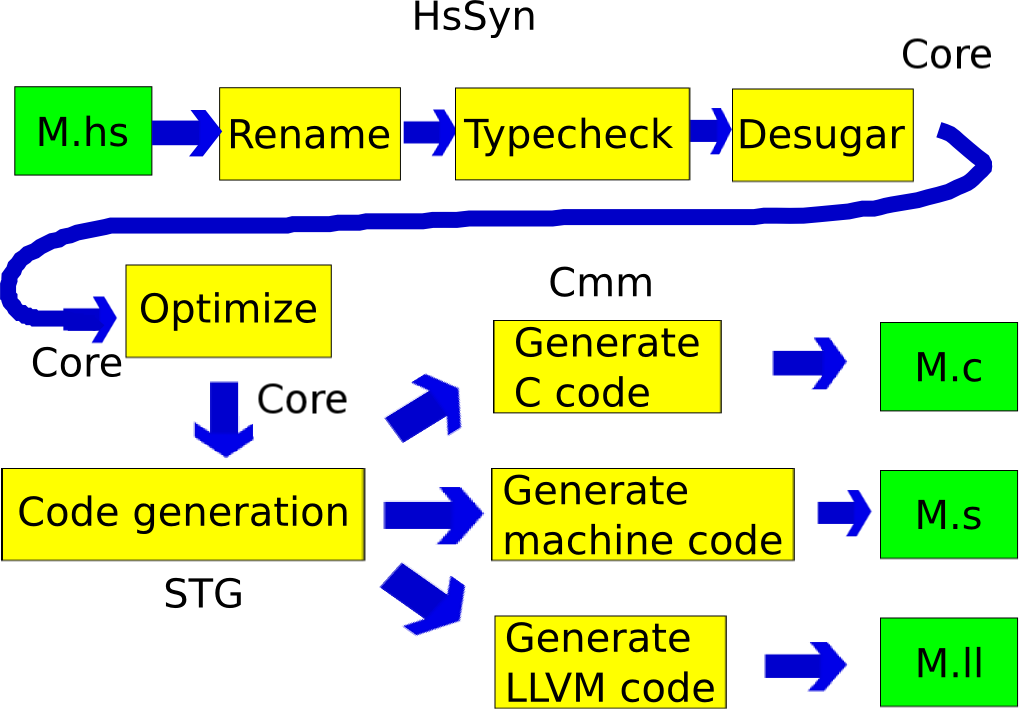
\includegraphics[width=0.6\textwidth]{images/ghc.png}
  \end{figure}

  \begin{itemize}
    \item Core: \enquote{$\lambda$-Kalkül mit Extras}, für Optimierungen
    \item STG: Spineless Tagless Graph-Machine, für Codeerzeugung
    \item Cmm: \enquote{C minus minus}, für Codeerzeugung
    \item Ca. 600.000 Zeilen Code, $\frac{3}{4}$ davon Haskell (selbst gezählt)
  \end{itemize}
\end{frame}

\section{propalang}

\begin{frame}{propalang}
  \code{code/propalang.pp}

  \begin{itemize}
    \item \href{https://pbrinkmeier.de/propalang.zip}{pbrinkmeier.de/propalang.zip}
    \item Im Repository: demos/java/propalang
    \item Parser für Expressions und Statements
    \item Interpreter: \texttt{java Main -- run test.pp}
  \end{itemize}
\end{frame}

\begin{frame}{propalang: Aufgaben}
  \code{code/propalang.pp}

  \begin{itemize}
    \item Erweitert den Parser um eine Divisionsoperation \texttt{/}
    \begin{itemize}
      \item \texttt{new OperatorExpression(Operator.DIVIDE, ...)}
    \end{itemize}
    \pause
    \item Erweitert den Parser um Schleifen \texttt{while} und \texttt{for}
    \begin{itemize}
      \item \texttt{while (condition) loopStmt;}
      \item \texttt{for (init; condition; post) loopStmt;}
      \item \texttt{new WhileStatement(...)}
      \item Keine neue AST-Klasse für \texttt{for}!
    \end{itemize}
  \end{itemize}
\end{frame}

\section{Ende}

\begin{frame}{Letzte Folie}
  \begin{itemize}
    \item Morgen, Mi, 09.02. um 14:00: Letzte Vorlesung
    \item ÜB-Korrekturen: Bis spätestens Ende Februar
    \item Klausur: 08.04.2022, 12:00
    \item Tutoriumsfolien, -code, etc.: \href{https://github.com/pbrinkmeier/pp-tut}{github.com/pbrinkmeier/pp-tut}
    \item Fragen auch gerne an \texttt{pp-tut@pbrinkmeier.de} :)
  \end{itemize}

  \vfill

  Danke fürs Kommen und eine gute Prüfungsphase!
\end{frame}

\end{document}
